%!TEX root = ../../main.tex

\chapter{Basics}
\section{Processing Units}
Processing Units are the central and most important part of a computer. The processing unit executes the instructions, is responsible for memory and communication and overall execute the program, that is given to the computer. Processing units consist of a Control Unit, Memory, Arithmetic Logical Unit and I/O elements. All of these parts together form a processing unit capable of performing many different instructions, mathematical operations, memory operations and much more. A basic overview of a processing unit is displayed in following graphic:\\
\begin{center}
	\begin{figure}[H]
		\centering
	\begin{tikzpicture}
		\draw (0,0) rectangle  (10,3);
		\draw (1,0.5) rectangle node{Memory}(3,2.5);
		\draw (3.6,0.5) rectangle node{\small Control Unit}(6.4,2.5);
		\draw (7,0.5) rectangle node{ALU}(9,2.5);
		\draw (4,3.5) rectangle node{Input}(6,5.5);
		\draw (4,-0.5) rectangle node{Output}(6,-2.5);
		\draw[very thick] [<->] (3,1.5) -- (3.6,1.5);
		\draw[very thick] [<->] (6.4,1.5) -- (7,1.5);
		\draw[very thick] [<->] (5,2.5) -- (5,3.5);
		\draw[very thick] [<->] (5,0.5) -- (5,-0.5);
	\end{tikzpicture}
\caption{Processing unit block diagram}
\end{figure}
\end{center}
\clearpage
The tasks and functionality of the different parts of a processing unit are described more closely in the dedicated section in chapter \ref{chapter:edrico}.\\
During the long history of computers and processors, different architectures have evolved. This section will give a quick overview of the so called \textit{Von-Neumann-Architecture} and the \textit{Harvard-Architecutre}.\\
The main difference between those two architectures is the memory access. While a Von-Neumann machine has a commonly used memory for data memory and program memory, a Harvard machine has separately dedicated memory units. This means, a Harvard machine can access to the program memory and the data memory simultaneously. The advantage of a Von-Neumann machine is that there is no limitations on how big the code and the data is. Sometimes, the program takes a lot of memory while the data amount only is very small and sometimes its the other way around. However with a Von-Neumann machine this is not a problem since the memory is used for program and data. In comparison to a Harvard machine, it would be bad to waste a lot of memory space, if the program only takes very little space or the other way around.\\
However, this advantage of the Von-Neumann architecture is a disadvantage at the same time, since some operations will take much longer than on Harvard machines, because memory cannot be accessed directly after loading an instruction.\\
In general it can be said, that the Von-Neumann architecture is more simple than the Harvard architecture, but the advantages it originally offered are nowadays solved with several principles and methods using the Harvard architecture. Nowadays, the Harvard architecture is used especially for applications where program size and data size are already known, which often is the case for embedded systems like digital signal processing units etc..\\
For this project, due to the big complexity of a Harvard architecture, the Von-Neumann architecture is implemented using a shared memory for program and data. \cite{hellmann2013}
The block diagrams of the two different architectures are displayed in following figures \ref{fig:neumann}, \ref{fig:harvard}:
\begin{figure}[H]
	\centering
	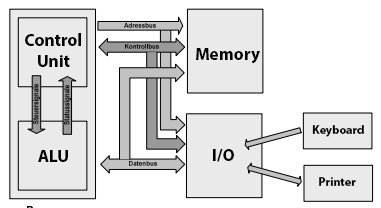
\includegraphics[width=\textwidth]{neumann.png}
	\caption{Von-Neumann architecture \cite{hellmann2013}}
	\label{fig:neumann}
\end{figure}

\begin{figure}[H]
	\centering
	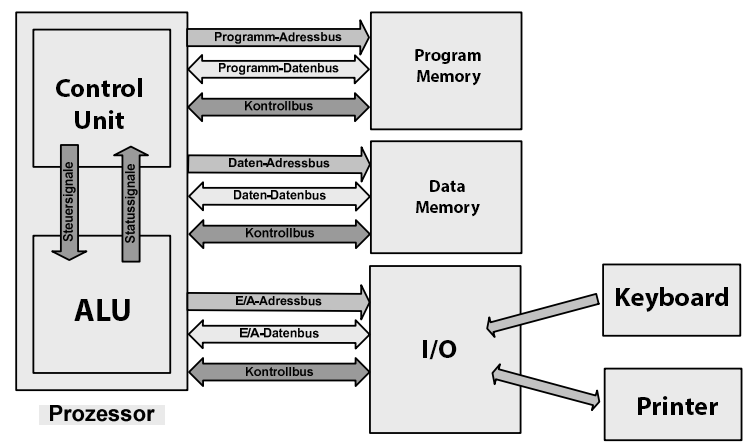
\includegraphics[width=\textwidth]{harvard.png}
	\caption{Harvard Architecture \cite{hellmann2013}}
	\label{fig:harvard}
\end{figure}


\section{RISC vs CISC}
In the history of processors and computers, speed and efficiency have always been key factors for development and innovation. In the early days of computers, instructions were very simple and straight forward. Coming with time and innovation, instructions and computer architectures became more complex. To prevent instructions from becoming too complex and too big, the \acf{RISC} architecture was introduced. The main point of RISC is to have a small but highly optimized set of instructions. Another advantage of RISC is a broadly uniform format of instructions and the possibility to establish pipelining which means starting the next instruction while the previous is being executed.\\
On the other hand, \acf{CISC} machines can have special instructions and more complex instructions to perform many things in one instruction cycle. However, the CPI can get greater than the CPI at for RISC architectures. Since the complexity of instructions increases, the time and computing effort increases as well. In CISC architectures, instructions do not have a standardized format and therefore, can differ in size and complexity. It is also possible to envelope microcode inside of instructions. This means that small pieces of programming can conclude small programs. Since instructions are very individual and not highly optimized, the amount of instructions can get very large. The differences between the two architectures are summarized in table \ref{table:riscvscisc}:
\begin{table}[H]
	\setlength\arrayrulewidth{2pt}
	\centering
	\resizebox{\textwidth}{!}{
		\begin{tabular}{|l|l|}
			\hline
			\rowcolor{light-gray}
			\textbf{RISC} & \textbf{CISC}\\
			\hline
			Single-cycle instructions & Instructions can take several clock cycles\\
			\hline
			Software-centric design: & Hardware-centric design:\\
			- High-level compilers take most action & - ISA does as much as possible using hardware circuitry\\
			\hline
			Simple, standardized instructions & Complex and variable length instructions\\
			\hline
			One layer instructions & Support microcode\\
			\hline 
			Small number of fixed-length instructions & Large number, variable sized instructions\\
			\hline
		\end{tabular}}
	\caption{RISC vs CISC \cite{hellmann2013}}
	\label{table:riscvscisc}
\end{table}
\clearpage
\section{RISC-V}
RISC-V is an open standard \acf{ISA} developed by the
University of California, Berkely. The ISA is based on reduced instruction set
computer (RISC) principles. The ISA supports 32, 64 and 128 bit architectures and
includes different extensions like Multiplication, Atomic, Floating Point and more. The
ISA is open source and therefore can be used by everyone without licensing issues
and high fee requirements. Due to the open source nature of the RISC-V project,
many companies like Alibaba and NVIDIA have started to develop hardware based
on this ISA.
RISC-V opens the opportunity to optimize and configure computer hardware to a
level that would not be realizable with licensed ISA like ARM or x86. As a result of
this possibility there are many projects and companies working on hardware and
software that are beating common CPU in terms of performance and power usage
by a lot.

\section{Benchmarks}
Benchmarks are measurement methods to evaluate performance of a computer. To measure benchmarks, a testing system is required. This testing environment is often established by using pre defined code or programs. These programs then are compiled and executed. The time this process takes is measured. The goal of a benchmark is to establish a certain comparability between different computers and processing units. \cite{gessler2014}\\
Working with benchmarks, a few principles have to be kept in mind. These vital characteristics of benchmarks are \cite{kounev2020systems}:
\begin{enumerate}
	\item \textbf{Relevance}: Only measure relevant features
	\item \textbf{Representativeness}: The metrics should be broadly accepted by industry and academia
	\item \textbf{Equity}: fair comparison of all systems
	\item \textbf{Repeatability}: Verification of results
	\item \textbf{Cost-effectiveness}: Tests are economical
	\item \textbf{Scalability}: Tests should work for systems with different range of resources
	\item \textbf{Transparency}: Metrics should be easy to understand
\end{enumerate}
There are several commonly used benchmarks depending on the type of system to be measured.\\
A very popular \ac{CPU} benchmark is the \textit{SPEC CPU}. This benchmark is being released ever since 1998 and gets updated and extended every couple of years. The most recent version is the \textit{SPEC CPU2017}. This benchmark suite concludes a lot of different benchmarks for different use-cases. The suite differs between \textit{rate} and \textit{speed} benchmarks and offers \textit{integer} as well as \textit{floating point} tests. The following table \ref{table:cpu2017} gives a brief overview of a few examples and their characteristics (only integer speed benchmark):
\begin{table}[H]
	\setlength\arrayrulewidth{2pt}
	\centering
	\resizebox{\textwidth}{!}{
		\begin{tabular}{|l|l|l|l|}
			\hline
			\rowcolor{light-gray}
			\textbf{Name} & \textbf{Language} & \textbf{\ac{KLOC}} & \textbf{Application}\\
			\hline
 			\textit{602.gcc\_s} & C & 1,304 & GNU C compiler \\			
			\hline
 			\textit{625.X264\_s} & C & 96 & Video compression \\	
 			\hline
 			\textit{631.deepsjeng\_s} & C++ & 10 & Artificial Intelligence: alpha-beta tree search \\	
 			\hline
	\end{tabular}}
	\caption{SPEC CPU2017 benchmark suite \cite{kounev2020systems}}
	\label{table:cpu2017}
\end{table}

 In this thesis, the main focus will be on the so called $\langle$\textit{Coremark}$\rangle$ and $\langle$\textit{SPECint}$\rangle$ benchmarks.
\subsection{CoreMark}
CoreMark is a openly available benchmark released by the \ac{EEMBC}. The CoreMark benchmark provides a starting point for measuring a processor's core performance. This allows the CoreMark to evaluate a wide range of different devices.\\
The workload of the CoreMark benchmark contains several algorithms like matrix manipulation, linked list manipulation, state machine operation etc. This mix of operations offers a realistic mixture of load and store, integer and control operations.\\
The benchmark itself performs following operations for the different benchmarks methods:
\begin{enumerate}
	\item \textbf{Linked List}: Perform multiple find operations (might end up traversing the whole list), sorting using merge sort (based on the value) and then derive a checksum of the data, sort again using merge sort (based on the index)
	\item \textbf{Matrix Multiply}: 3 matrices A,B,C (NxN size): 
	\begin{enumerate}
		\item Multiply A by a constant into C
		\item Multiply A by column X of B into C
		\item Multiply A by B into C
	\end{enumerate}
	\item \textbf{State Machine}: Perform \textit{switch} and \textit{if} statements using a Moore state machine:\\
	parse an input string, extract number $\rightarrow$ if valid number $\rightarrow$ return\\
	Modify input at intervals and invoke state machine on all states
\end{enumerate}
Since CoreMark is an openly available benchmark, some license agreements have to be met and also there is a strict rule for reporting the results of a benchmark. These results have to be published and consist of:
\begin{itemize}
	\item \textbf{N}: Number of iterations per second
	\item \textbf{C}: Compiler version and flags
	\item \textbf{P}: Parameters such as data and code allocation specifics
	\item \textbf{M}: Type of parallel algorithm execution (if used)
\end{itemize}
\subsection{SPECint}
SPECint is a computer benchmark specification for CPU integer processing power. In this section, the SPECint2006 suite is described in detail. The SPECint2006 suite consists of 12 programs where each is compiled and run three times. The runtimes are measured and the median is used to calculate a runtime ratio. This means that the benchmark compares the measured time to a reference run time. A mathematic aproach for this calculation is given in following formula:
$ ratio_{program} = \dfrac{T_{ref}(program)}{T_{SUT}(program)} $ with\\
$ T_{ref}(program) $ = runtime of the specific program on the reference machine\\
SUT = system under test\\
$ T_{SUT}(program) $ = runtime of the specific program on SUT\\
Therefore, ratios are higher for faster machines, and lower for slower machines. To determine the whole SPECint2006 score, the geometric mean of all 12 rations is computed. The 12 programs of the SPECint2006 benchmark are displayed in the following table \ref{table:spec2006int}:
\begin{table}[H]
	\setlength\arrayrulewidth{2pt}
	\centering
	\resizebox{\textwidth}{!}{
		\begin{tabular}{|l|l|l|}
			\hline
			\rowcolor{light-gray}
			\textbf{Program} & \textbf{Language} & \textbf{Category}\\
			\hline
			\textit{400.perlbench} & C & Perl Programming language\\			
			\hline
			\textit{401.bzip2} & C & Compression \\	
			\hline
			\textit{403.gcc} & C & C Compiler \\	
			\hline
			\textit{429.mcf} & C & Combinatorial Optimization \\	
			\hline
			\textit{445.gobmk} & C & Artificial Intelligence: go playing (complex computer game) \\	
			\hline	
			\textit{456.hmmer} & C & Search Gene Sequence \\	
			\hline	
			\textit{458.sjeng} & C & Artificial Intelligence: chess playing \\	
			\hline
			\textit{462.libquantum} & C & Quantum Computing \\	
			\hline
			\textit{464.h264ref} & C & Video Compression \\	
			\hline
			\textit{471.omnetpp} & C & Discrete Event Simulation \\	
			\hline
			\textit{473.astar} & C & Path-finding Algorithms \\	
			\hline
			\textit{483.xalancbmk} & C & 	XML Processing \\	
			\hline
	\end{tabular}}
	\caption{SPECint2006 programs \cite{specint}}
	\label{table:spec2006int}
\end{table}

\section{Memory Management}
Memory Management defines how the memory can be accessed and how changes propagate through different levels of the memory hierarchy. The following section will describe what a memory hierarchy is and why it is needed in modern computer designs. Furthermore one particular communication interface or bus system will be introduced which can be used to access memory in an embedded system. 
\subsection{Memory Hierarchy}
One of the major performance factors in computing is how fast can information be accessed. Information in this case is both: data and code. Therefore high-speed infinite sized memory would be the optimum to achieve the best possible performance. Unfortunately multiple difficulties are raised by this requirement. How can an infinite sized memory be achieved, how to guarantee that access time does not increase when increasing the memory size and how to keep costs to minimum are only a few of the many questions that can be asked on this topic.\\
In general it can be said that infinite sized memory is not possible, therefore the new requirement would be: as big as possible. To achieve low access times, the memory must be placed as close as possible to the processor. The amount of extremely fast memory is therefore restricted to a finite size. Increasing the distance to the processor yields more space, hence a bigger possible memory. Access speed is reduced at the same time.\\
Therefore the only way to have a big high-speed memory is to emulate it. This is done by taking advantage of two principles: temporal- and spatial locality \cite{patterson:2017}. 
Temporal locality suggests that data which is accessed will be used again in the near future. This can be caused by loops inside a routine. 
Spatial locality is very similar. If data from one particular region is accessed, there is a high probability of an access to the same region in the near future. Many data structures, for example arrays, cause spatial locality.\\
Figure \ref{fig:memHierarchy} shows an example of a possible memory hierarchy: 

\begin{figure}[h]
	\centering
	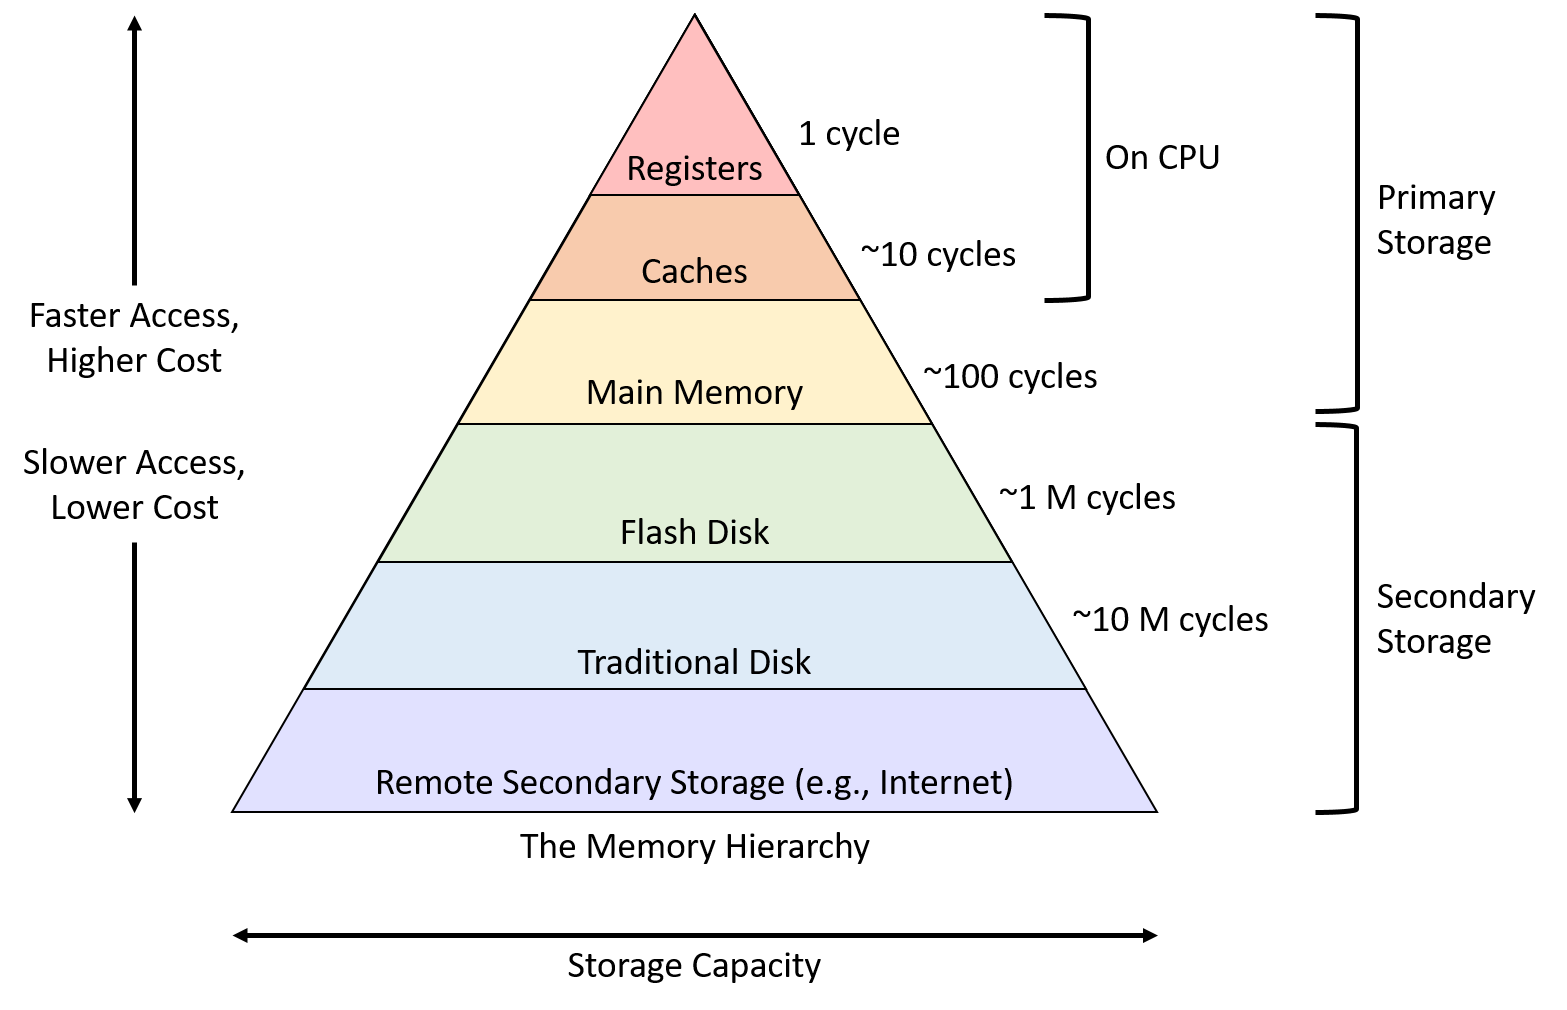
\includegraphics[width=\textwidth]{MemoryHierarchy.png}
	\caption{Generic Memory Hierarchy \cite{picture:memoryhierarchy}}
	\label{fig:memHierarchy}
\end{figure}
 
The closer a memory element is placed to the processing unit, the faster it gets. This is not only caused by the spatial distance but also by the chosen memory type. For example registers are the closest, followed by SRAM which is typically used for L1,L2 and sometimes even L3 caches \cite{patterson:2017}.\\
If a memory access is performed, the memory management system first checks whether or not the desired data is stored in the upper memory levels. A hit occurs when the data block is found in an upper level of the memory hierarchy. In case of a miss, the search for the required data block is continued in the lower levels. If it is found e.g. in main memory, the data will be provided to the processor and copied into the cache. Therefore satisfying the temporal locality principle. Surrounding data blocks are also copied to the cache in order to prevent another miss in case of spatial locality.\\
Performance of the memory hierarchy can be measured by the hit and miss rate. These describe the portion of miss and hits of the overall memory accesses. Miss rate can be calculated, if the hit rate is known:

$$miss rate = (1 - hit rate)$$

To get a significant measurement of the performance, hit time and miss penalty have to be considered as well. The hit time is defined as the time it takes to get the data block from the cache if a hit occurs. After a miss is detected, that block of data has to be retrieved from main memory, stored in the cache and provided to the processor. The overall time required for these three steps is defined as the miss penalty \cite{patterson:2017}.\\
Different ways of increasing cache performance are described in \cite{patterson:2017}.\\


\subsection{Communication Interfaces}
\label{chapter:axiCommInterfaces}
In order to access memory, some sort of communication interface / bus system is required. There are countless options like the widely used \ac{PCIe} and \ac{CAN} bus or application specific systems, e.g. SpaceWire used in satellite systems or \acp{ARM} \ac{AMBA}.\\
The following section will provide an overview of the \ac{AXI4-Lite} protocol which is implemented in the \ac{EDRICO}.\\
An AXI interface has four independent channels: read address, write address, read data, write data and write response. Figure \ref{fig:AXI_channels_write} and \ref{fig:AXI_channels_read} visualizes these three channels:

\begin{figure}[H]
	\centering
	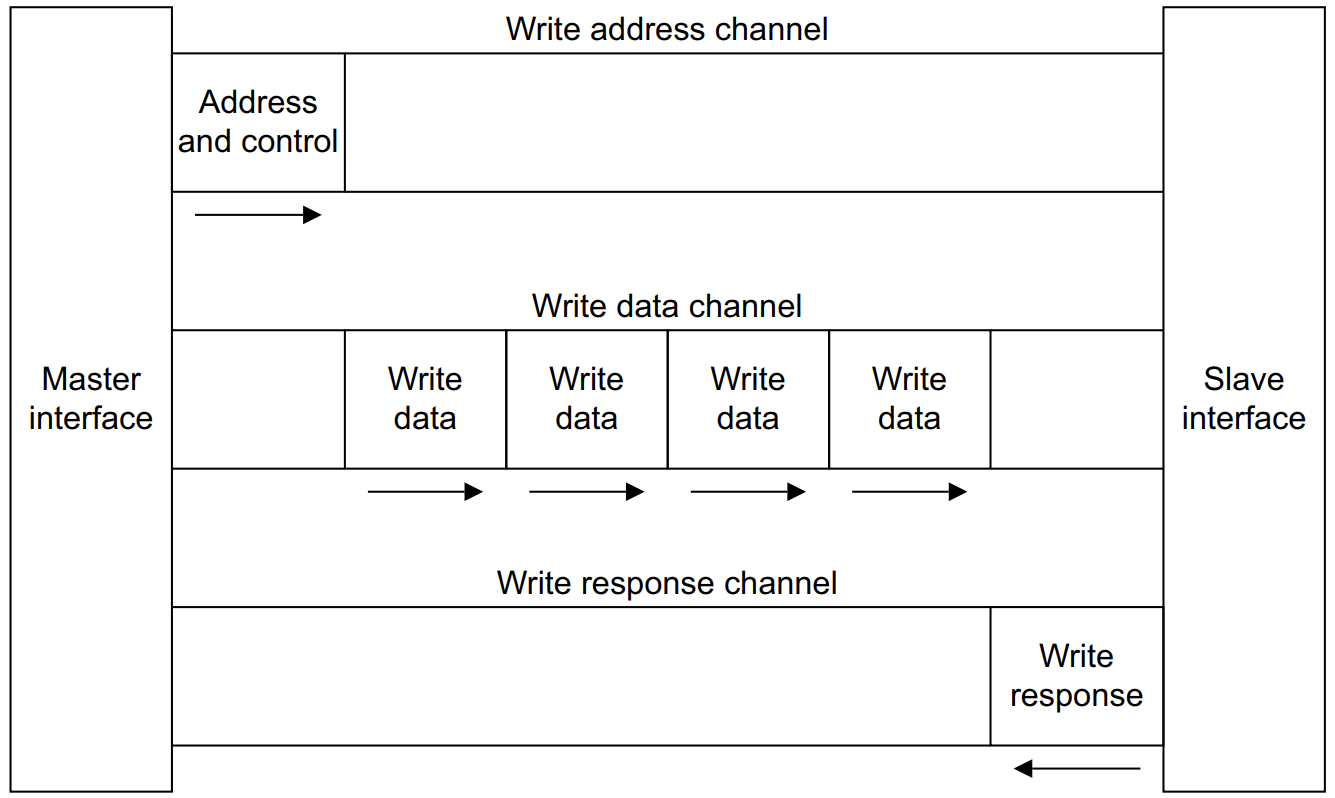
\includegraphics[width=\textwidth]{AXI4_write.png}
	\caption{\ac{AXI}4 write channels \cite{AMBA:AXI}}
	\label{fig:AXI_channels_write}
\end{figure}

\begin{figure}[H]
	\centering
	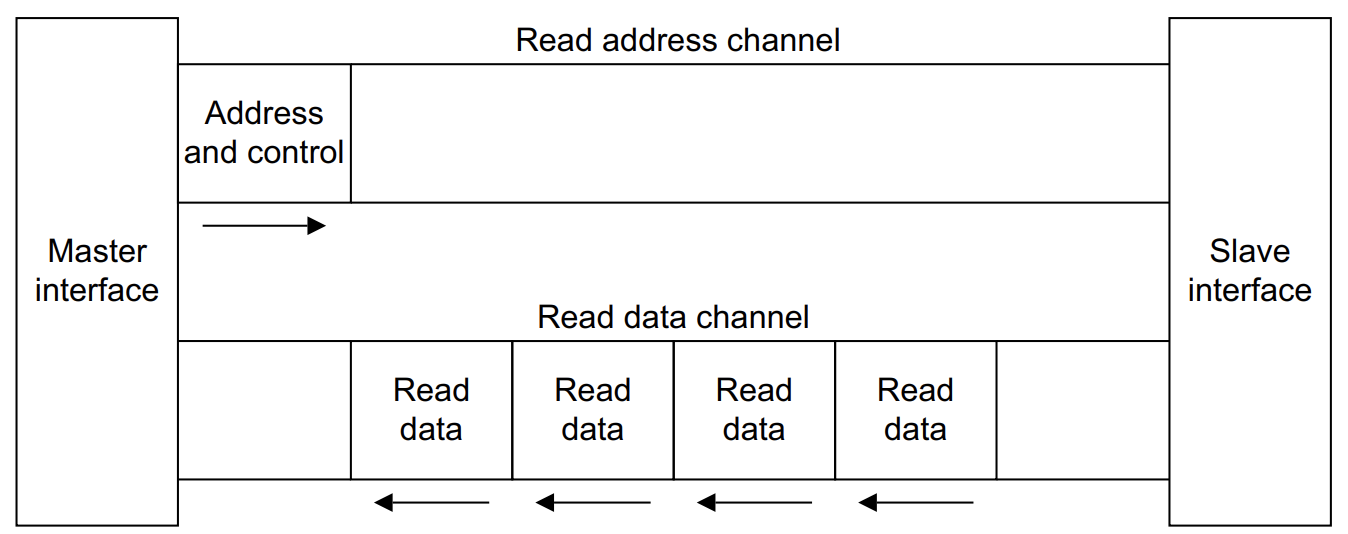
\includegraphics[width=\textwidth]{AXI4_read.png}
	\caption{\ac{AXI}4 read channels \cite{AMBA:AXI}}
	\label{fig:AXI_channels_read}
\end{figure}

The master interface always initiates the transaction by sending either the write or read address and control. In case of a write, the data is send to the slave using the write data channel. A response is given by the slave, containing information on the transfer. The slaves response on a read does not need a separate channel, since it can be transmitted using the read data channel.\\
AXI4-Lite does not support burst transfers, hence only one data word can be transmitted in one transfer. To transfer any data over any channel, a generic handshake process must be completed. Figure \ref{fig:AXI_handshake} shows how the handshake is performed:

\begin{figure}[H]
	\centering
	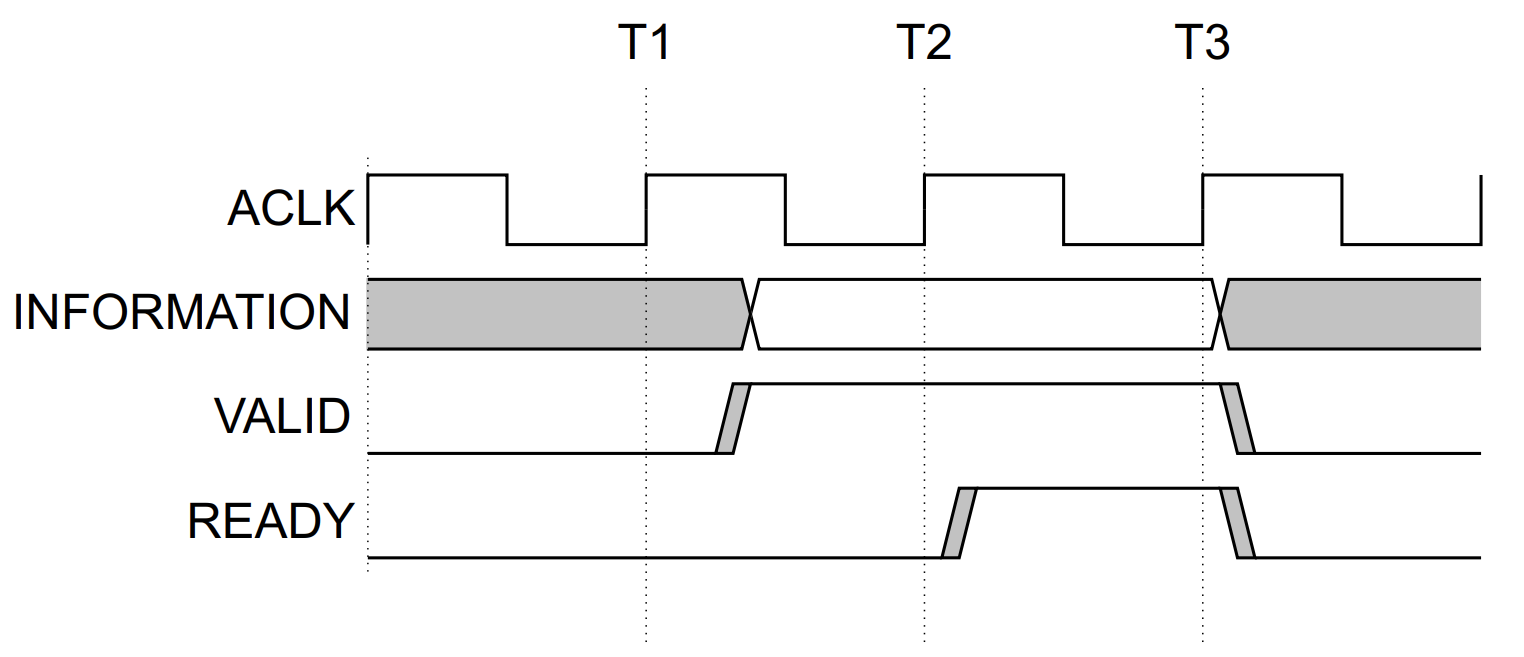
\includegraphics[width=\textwidth]{AXI_handshake.png}
	\caption{\ac{AXI} handshake \cite{AMBA:AXI}}
	\label{fig:AXI_handshake}
\end{figure}
 
At transfer begin, the sending interface applies the information (e.g. the read address) on the bus. The Valid signal indicates that the information is valid, it must stay valid until the receiving interface applies the ready signal. Ready indicates that the receiving partner is ready to receive the information. If both signals (valid and ready) are high on a rising clock edge, the information is read by the receiver and the flow control signals are tied to low \cite{AMBA:AXI}. This handshake mechanism allows the receiving \ac{AXI} interface to extend the length of the transfer when needed. Since each of the five \ac{AXI}4 channels are independent five handshake mechanisms are implemented.\\
A response of a slave contains the \textit{RRESP} or \textit{BRESP} signals, respectively. They can be set to OKAY, EXOKAY, SLVERR, and DECERR. In case of an okay or exclusive okay, no error has occurred. SLVERR indicates that an error has occurred on the slave side, even though the slave successfully registered the access. If no slave is available on the interrogated address, a DECERR is returned.\\\\
Based on the response of the slave, a masters behavior must adapt. If (EX)OKAY is returned it may proceed normal operation. If an error is detected error handling methods such as exceptions must be triggered. \\
The \ac{AMBA} protocols are widely used in embedded systems. Many \acp{IP} deployed in \acp{FPGA} can be interfaced using the \ac{AXI}4 or \ac{AXI4-Lite} bus. Therefore it is mandatory to be familiar with this particular bus architecture when working with embedded systems.




\section{FPGA}
To verify a digital circuit software simulations as well as implementing the design on
a prototype are common practice. For prototyping and even implementing a finished
product, \acp{FPGA} are widely used.
\acp{FPGA} are special fine granularity programmable logic devices. The digital logic
can be described using hardware description languages such as Verilog or \ac{VHDL}.
These designs are then synthesized, placed and routed in order to generate a
hardware configuration file, also called bitstream. The bitstream can then be loaded
onto the \ac{FPGA} via a programming interface e.g. \ac{JTAG}.
Many different vendors produce \acp{FPGA}, the most famous ones are Xilinx,
Altera/Intel and Microchip. Some smaller vendors like NanoXplore produce \acp{FPGA}
targeting rare use cases like space applications.
Despite the many differences in design, the basic architecture always
remains the same. An array of logic cells and building blocks of different features
like \ac{BRAM} and \ac{DSP} slices are connected to each other through configurable routing
channels \cite{kesel:2018}.
Figure \ref{fig:FPGA} shows the basic architecture of a Xilinx \ac{FPGA}:\\

\begin{figure}[h]
\centering
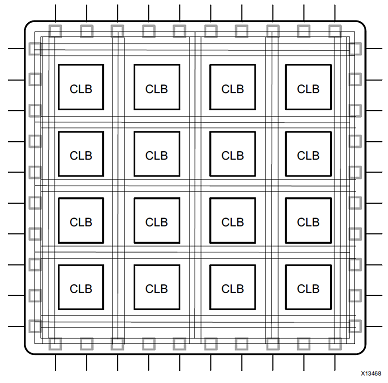
\includegraphics[scale=0.7]{fpga.png}
\caption{Xilinx FPGA \cite{xilinx:2017}}
\label{fig:FPGA}
\end{figure}
\section{Hardware Description Languages}
A \acf{HDL} is a computer language specialized to describe structure and behavior of electronic circuits. HDLs were created to implement register-transfer level abstraction which is a model of the data flow and timing of a circuit.\\
HDL can be used to express designs in structural, register-transfer-lever or behavioral architectures for a specific functionality.\\
VHDL is a description language used to describe hardware. It is utilized in electronic design to express digital systems such as integrated circuits and FPGA. VHDL is also used as a general-purpose parallel programming language. VHDL is used to write text models that describe or express logic circuits. If the text model is part of the logic design, the model is processed by a synthesis program. Implementation and testing of VHDL is described more closely in following chapters. The critical advantage of VHDL, with regard to system design utilization is that it permits the behavior of the essential system to be verified and modeled in advance of the synthesis tools translation of the design into actual hardware. In addition, it is a dataflow language, which means it can simultaneously consider every statement for execution other than procedural computing languages like C. As a last advantage to be mentioned here, VHDL projects can be multipurpose. It is possible to create units and blocks and re use them for other applications.\\
Another HDL on the market is Verilog. Verilog is a more compact language and often results in less lines of code and is more similar to programming languages like C. However, Verilog is not as wordy as VHDL, which accounts for its compact nature. Verilog also is more of a hardware modeling language and not so natural in use as VHDL. Nonetheless, Verilog is often considered as easier to learn. 


